\subsection{Absolute Polarization Angle}

\paragraph{Description:}
Absolute Polarization Orientation refers to the polarimeter detectors'
direction measured in celestial coordinates. A miscalibration (i.e. a rotation
bias for the detector orientation) mixes E-modes and B-modes. In addition to
contaminating the CMB polarization power spectra, such a systematic rotation is
degenerate with Cosmic Birefringence (CB) and Cosmic Polarization Rotation
(CPR).

Sources of polarization angle systematics are varied and can be introduced
several places in the instrument. A few examples include 1) a rotating
elliptical beam, say in the case of a design incorporating bore-sight
rotations, causing T to P leakage (see ellipticity section); 2) off-axis
refractive optics influencing the propagation of the polarization vectors
according to their Fresnel coefficients, leading to an instrumental
polarization angle rotation; and 3) an apparent polarization angle rotation
from the detector time constants in the presence of a HWP (see time constant
section). Here we focus on 2), namely instrumental polarization errors and
detector polarization angle rotations.

A global polarization rotation is degenerate with a CPR angle and affects the
power spectra as described in \cite{2013ApJ...762L..23K}. Analytic description
of instrumental rotation is challenging, necessitating the use of optical
modeling and experimental techniques for calibration of final detector angles
(absolute and relative) and systematic rotations from the optics.

\paragraph{Plan to model and/or measure:}
It is critical to both model and measure the detector polarization angles.
Calibration should be performed before deployment and during observations. 
We plan to use polarization calibrators in-lab while testing full optics tubes
before deployment, in situ in the field with polarization calibrators (either
drone/ground-based), and observations polarized astrophysical sources like Tau
A (the Crab Nebula) and Cen A \textbf{give some citations}.

When considering a lab source, placing a well known polarization calibrator in
the far field is preferred, though difficult in practice.  Proposed ideas
include artificial sources \cite{nati_2017} (whether tunable or wide band)
flying on a drone or on balloon or a CalSat to place them in the far field.
Alternative calibrators require placement in the near field and include
sparse/dense wire grid polarizers or dielectric sheets \cite{Takahashi2010,
2016arXiv160701825K}. \textbf{Say something about the PB calibrator that Grant
has been working on, something about PoloCalc, and other options. Note that it
would be easier to measure in-lab if we only have the optics tubes and what
options we have for that. See the calibration hardware spreadsheet linked on
the CSS telecon page.}

Modeling of the polarization rotation angle appears feasible and has been used
on ACTPol using Code V \cite{2016arXiv160701825K}. Polarization rotation can be
modeled in CODE V using a polarization sensitive ray trace. An input
polarization is defined and propagated through the optical chain to the
detector focal plane. The pupil averaged Stokes vector is then used to
calculate the polarization angle at the focal plane. This process is repeated
for 25 different fields on the sky and the results are fit to a 2D quadratic.
This fit is then used to estimate the rotation for each detector on the focal
plane. An example of the modeled rotation for the first Advanced ACT array is
shown in Figure \ref{fig:advact_pa4_pol_rotation}. A similar analysis can be
done in Zemax, though is known to not be accurate for fast optical systems.

\begin{figure}[h!]
\begin{center}
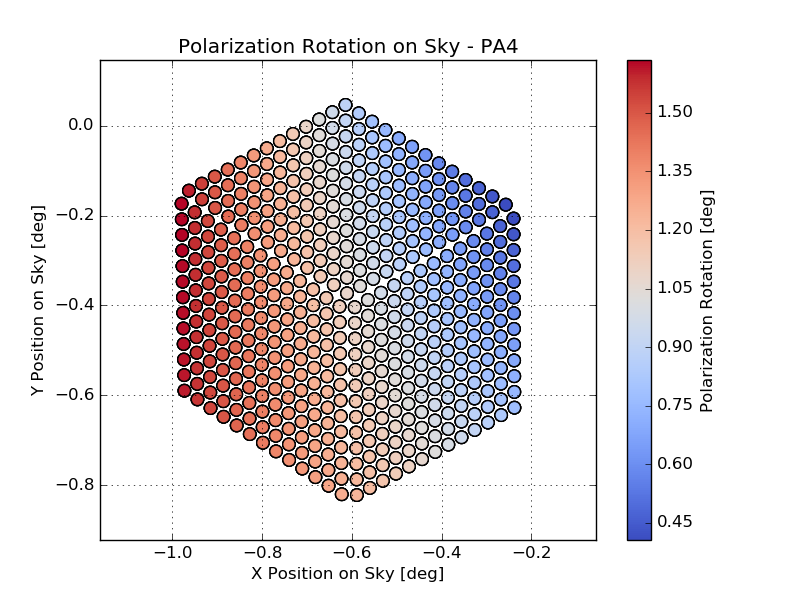
\includegraphics[width=0.60\linewidth]{advact_pa4_polarization_rotation_150ghz_2017.png}
\caption{Modeled instrumental polarization rotation for the high frequency (HF)
Advanced ACT array. Each circle represents a single feedhorn at the focal
plane. The color represents the amount of rotation as modeled by CODE V.}
\label{fig:advact_pa4_pol_rotation}
\end{center}
\end{figure}

This should be checked with physical optics calculations and measurements, but
can be performed on a proposed telescope design which includes both reflectors
and lenses.

\textbf{Can we use EB and TB cross-crrelations to help in our null tests for
absolute polarization angle?}

Understanding the polarization anlge is critical to achieving several science
goals and thus has an SRF of 5.

\paragraph{Uncertainty/Range:}
%This section should include the uncertainty of
%known parameters and/or the expected range of parameters for consideration

Angle offsets $\sim 1^{\circ}$ produce spurious B-mode signal at the same level
as primodial B-modes for a tensor to scalar ratio of $r \sim 0.005$ as well as
nonzero $EB$ and $TB$ cross-correlations \cite{doi:10.1142/S0218271816400125}.
\textbf{Say what the r goal for SO is, and what angle calibration that
requires.} Currently employed calibration methods provide calibration to at
best $0.5^{\circ}$ \cite{2016MNRAS.455.1981K} \textbf{Is this sufficient for
SO's science goals or do we need more R and D to reach our scienc goals?}.
Calibration to better than $0.05^{\circ}$ would allow for constraints on CPR of
order one degree to greater than $15\sigma$ \cite{2016MNRAS.455.1981K}
\textbf{What about on r?}.  \textbf{Use some of the plots and numbers from
Federico's paper here}

\paragraph{Parameterization:}
This effect can be parameterized by the polarization angle uncertainty, which
can be used to estimate the polarization power spectra leakages as in
\textbf{cite Federico's paper}. This can be used to estimate the impact on our
science goals.
